\clearpage
\section{\RU{Простейшее четырехбайтное XOR-шифрование}\EN{Simplest possible 4-byte XOR encryption}}

\RU{Если при XOR-шифровании применялся шаблон длинее байта, например, 4-байтный, то его также легко
увидеть.}
\EN{If longer pattern was used while XOR-encryption, for example, 4 byte pattern, it's easy
to spot it as well.}
\RU{Например, вот начало файла kernel32.dll (32-битная версия из Windows Server 2008):}
\EN{As example, here is beginning of kernel32.dll file (32-bit version from Windows Server 2008):}

\begin{figure}[H]
\centering
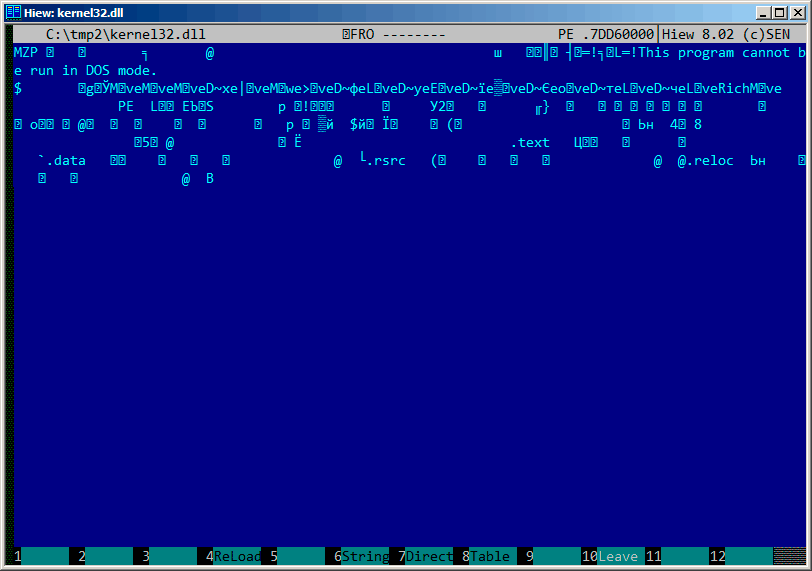
\includegraphics[scale=\FigScale]{ff/XOR/4byte/original1.png}
\caption{\EN{Original file}\RU{Оригинальный файл}}
\end{figure}

\clearpage
\RU{Вот он же, но \q{зашифрованный} 4-байтным ключем:}
\EN{Here is it \q{encrypted} by 4-byte key:}

\begin{figure}[H]
\centering
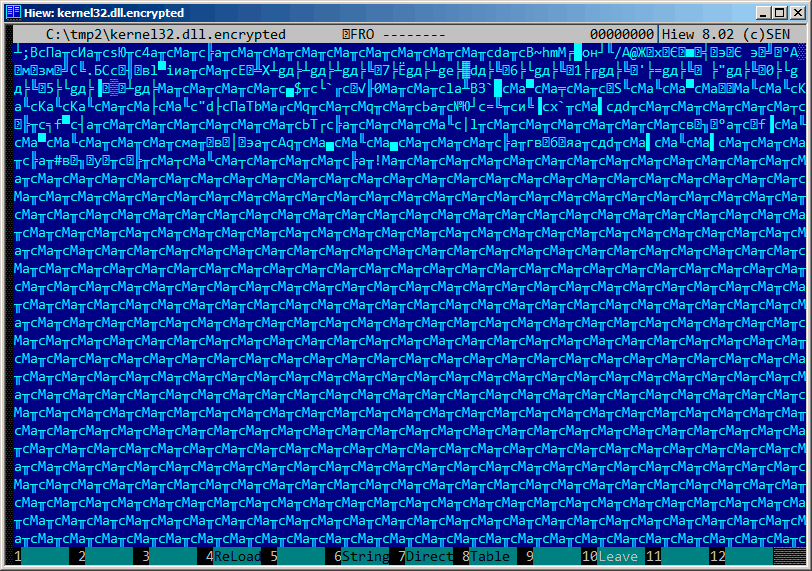
\includegraphics[scale=\FigScale]{ff/XOR/4byte/encrypted1.png}
\caption{\EN{\q{Encrypted} file}\RU{\q{Зашифрованный} файл}}
\end{figure}

\RU{Очень легко увидеть повторяющиеся 4 символа.}
\EN{It's very easy to spot recurring 4 symbols.}
\RU{Ведь в заголовке PE-файла много длинных нулевых областей, из-за которых ключ становится видным.}
\EN{Indeed, PE-file header has a lot of long zero lacunes, which is the reason why key became visible.}

\clearpage
\RU{Вот начало PE-заголовка в 16-ричном виде:}
\EN{Here is beginning of PE-header in hexadecimal form:}

\begin{figure}[H]
\centering
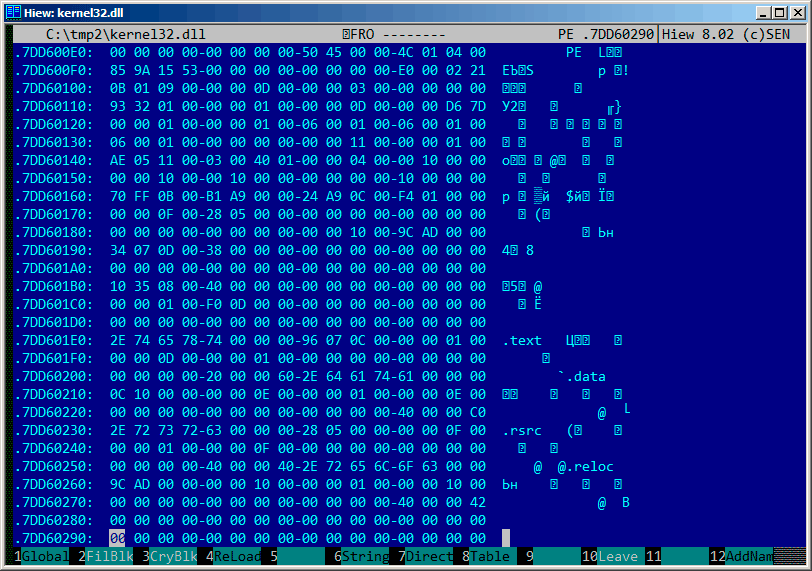
\includegraphics[scale=\FigScale]{ff/XOR/4byte/original2.png}
\caption{PE-\EN{header}\RU{заголовок}}
\end{figure}

\clearpage
\RU{И вот он же, \q{зашифрованный}:}
\EN{Here is it \q{encrypted}:}

\begin{figure}[H]
\centering
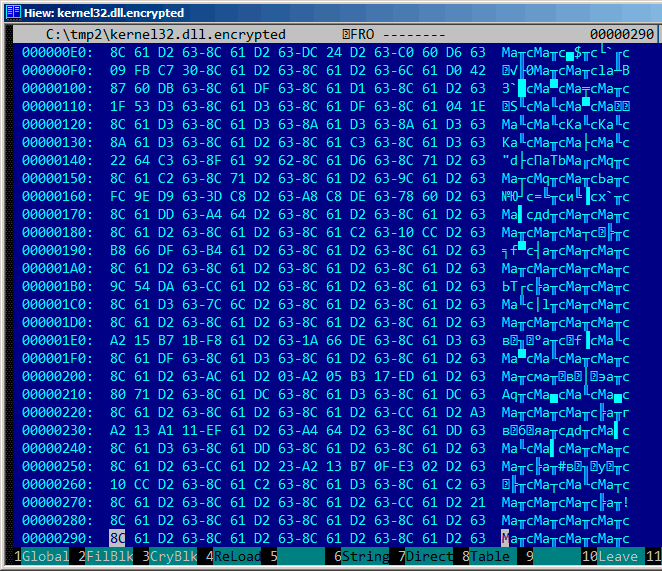
\includegraphics[scale=\FigScale]{ff/XOR/4byte/encrypted2.png}
\caption{\EN{\q{Encrypted} PE-header}\RU{\q{Зашифрованный} PE-заголовок}}
\end{figure}

\RU{Легко увидеть визуально, что ключ это следующие 4 байта}
\EN{It's easy to spot that key is the following 4 bytes}: \TT{8C 61 D2 63}.
\RU{Используя эту информацию, довольно легко расшифровать весь файл.}
\EN{It's easy to decrypt the whole file using this information.}

\RU{Таким образом, важно помнить эти свойства PE-файлов:
1) в PE-заголовке много нулевых областей;
2) все PE-секции дополняются нулями до границы страницы (4096 байт), 
так что после всех секций обычно имеются длинные нулевые области.}
\EN{So this is important to remember these property of PE-files:
1) PE-header has many zero lacunas;
2) all PE-sections padded with zeroes by page border (4096 bytes),
so long zero lacunas usually present after all sections.}

\RU{Некоторые другие форматы файлов могут также иметь длинные нулевые области.}
\EN{Some other file formats may contain long zero lacunas.}
\RU{Это очень типично для файлов, используемых научным и инженерным ПО.}
\EN{It's very typical for files used by scientific and engineering software.}

\RU{Для тех, кто самостоятельно хочет изучить эти файлы, то их можно скачать здесь:}
\EN{For those who wants to inspect these files on one's own, they are downloadable there:}
\url{http://go.yurichev.com/17352}.

\subsection{\Exercise}

\EN{As an exercise, try to decrypt the following file. Key is different, of course.}
\RU{В качестве упражнения, попробуйте дешифровать этот файл. Ключ другой, конечно.}
\url{http://go.yurichev.com/17353}.
